\documentclass[arial,english,brazil,oneside]{estiloifes}

\usepackage[utf8]{inputenc}
\usepackage{lastpage}           % Usado pelo exemplo de ficha catalográfica
\usepackage[alf]{abntex2cite}
\usepackage{microtype}          % para melhorias de justificação
\usepackage{morefloats}         % permite mais floats
\usepackage{listings}
\usepackage{blindtext}          % para gerar texto aleatório (dummy text)
\usepackage{tikz}
\usetikzlibrary[topaths]
\usepackage{mathtools}
\usepackage{float}
\usepackage{setspace}
\usepackage{quoting}
\usepackage{setspace}% http://ctan.org/pkg/{setspace,lipsum}






%\setlist{parsep=\parskip,leftmargin=1.5cm}
\renewcommand{\baselinestretch}{1.5}
%%% Definição da linguagem padrão do documento (pacote babel) para
%%% definir que certas porções do texto (como o resumo, por exemplo)
%%% estão em uma língua estrangeira, usar as macros
%%% \foreignlanguage{languageB}{Text in another language}
%%% ou
%%% \begin{otherlanguage}{languageB}
%%% ...
%%% \end{otherlanguage}
\selectlanguage{brazil}


%%% Define que todos os códigos fontes construídos com o ambiente
%%% `lstlisting' terão uma borda simples.
\lstset{frame=single}


\newcommand{\ifestex}{\textsf{Ifes$7$}}

\titulo{Arquitetura distribuída para APIs de Machine Learning}

\autor{Luan Grillo Silva}
\autorficha{Silva, Luan Grillo}

\orientador{DSc. Eros Moura}


\instituicao{IFES - Instituto Federal do Espírito Santo}

\curso{Bacharelado em Sistemas de Informação}

\data{2022}

\local{Cachoeiro de Itapemirim - ES}

\preambulo{Trabalho de Conclusão de Curso apresentado à Coordenadoria
  do Curso de Sistemas de Informação do Instituto Federal do Espírito
  Santo, Campus Cachoeiro de Itapemirim, como requisito parcial para a obtenção do
  título de Bacharel em Sistemas de Informação.}

\tipotrabalho{Trabalho de Conclusão de Curso}


\begin{document}



\imprimircapa

\imprimirfolhaderosto*

%\begin{fichacatalografica}
  \vspace*{\fill}
  % Posição vertical
  \begin{center}
    % Minipage Centralizado
    \fbox{
      \begin{minipage}[t]{12.5cm}
        \vspace*{3mm}
        \begin{minipage}[t]{2cm}
          X000x
        \end{minipage}
        \begin{minipage}[t]{10cm}
          \imprimirautorficha.\vspace{2mm}

          \hspace{0.5cm}\imprimirtitulo\ / \imprimirautor. ---
          \imprimirlocal, \imprimirdata.\\ 

          \hspace{0.5cm}\pageref{LastPage} p.:\ il. (algumas color.);
          30 cm.\\ 

          \hspace{0.5cm}\imprimirorientadorRotulo~\imprimirorientador.\\

          \hspace{0.5cm}\imprimirtipotrabalho\ ---
          \imprimirinstituicao, \imprimirdata\\

          \hspace{0.5cm}        
          1. Palavra-chave1.
          2. Palavra-chave2.
          I. Orientador.
          II. Universidade xxx.
          III. Faculdade de xxx.
          IV. Título.
          
          \begin{flushright}
            CDU 00:000:000.0
          \end{flushright}
          \vspace*{1mm}
        \end{minipage}
      \end{minipage}
    }
  \end{center}
\end{fichacatalografica}

%
%%% ====================================================================
%%% Exemplo de construção da folha de aprovação. Depois da
%%% apresentação do trabalho, quando a folha de apresentação real
%%% tiver sido assinada pela banca, a folha real deve ser digitalizada
%%% e o ambiente abaixo deve ser substituído por:
%%% \includepdf{folhadeaprovacao_final.pdf}
\begin{folhadeaprovacao}
  \begin{center}
    {\ABNTEXchapterfont\MakeTextUppercase{\imprimirautor}}\\
    \begin{center}
      \ABNTEXchapterfont\MakeTextUppercase{\imprimirtitulo}\\
    \end{center}
    \hspace{.45\textwidth}
    \begin{minipage}{.5\textwidth}
      {\footnotesize{\imprimirpreambulo}}\\
    \end{minipage}%
  \end{center}
  \vspace{-1cm}%
  \begin{center}
    Aprovado em 20 de Novembro de 2017.\\[15mm]
    \textbf{COMISSÃO EXAMINADORA}\\[5mm]
    \assinatura{\imprimirorientador \\
      Instituto Federal do Espírito Santo - Cachoeiro de Itapemirim \\ Orientador}\vspace{-1cm}
    \assinatura{DSc. Convidado 1 \\
      Instituto Federal do Espírito Santo - Cachoeiro de Itapemirim}\vspace{-1cm}
    \assinatura{DSc. Convidado 2\\
      Instituto Federal do Espírito Santo - Cachoeiro de Itapemirim}\vspace{-1cm}
  \end{center}
\end{folhadeaprovacao}
%%%% --------------------------------------------------------------------
%%% Ambiente para escrita da declaração do autor
\begin{declaracaodoautor}

  \vspace*{1.5cm}

  Declaro, para fins de pesquisa acadêmica, didática e
  técnico-científica, que este Trabalho de Conclusão de Curso pode ser
  parcialmente utilizado, desde que se faça referência à fonte e ao
  autor.

  \vspace*{2.5cm}

  \centering

  \imprimirlocal, 20 de Novembro de 2017.

  \vspace*{2.5cm}

  \imprimirautor

  \vspace*{\fill}
  
\end{declaracaodoautor}

%%%% ====================================================================
%%% Ambiente para a escrita da dedicatória.
\begin{dedicatoria}
  \vspace*{\fill}
  \hspace{0.2\textwidth}
  \begin{minipage}{0.8\textwidth}
 Dedico esse trabalho primeiramente a Deus e a todos que de alguma forma contribuíram  para que o mesmo fosse realizado.
  \end{minipage}
\end{dedicatoria}
%%%% ====================================================================
%%% Agradecimentos
\begin{agradecimentos}
Primeiramente agradeço a Deus...

\end{agradecimentos}
%%%% ====================================================================
%%% Epígrafe
\begin{epigrafe}
  \vspace*{\fill}
  \begin{otherlanguage}{english}
    \begin{flushright}
      \begin{SingleSpace}
       "Boop, boop, beep, boop, beep".\\ 
        R2D2
      \end{SingleSpace}
    \end{flushright}
  \end{otherlanguage}
\end{epigrafe}
%%% Ambiente para resumo em português
\begin{resumo}
    Esse artigo aborda uma pesquisa aplicada e desenvolvimento de arquitetura distribuída baseadas no padrão publish/subscribe empregada em dispositivos de Internet das Coisas (IoT). Visando alta escalabilidade e  e um baseia se principalmente na problemática de projetos que demandam de um grande aglomerado de dispositivos conectados para uso de atuadores ou captura de dados sensoriais, para isso, torna-se indispensavel utilização do padrão pub/sub em projetos IoT, viabilizando o custo do projeto e a simplificação de diversas partes desta arquitetura.

Palavras-chave:
Sistemas distribuídos, Publish/Subscribe, IoT, Computação distribuída



\end{resumo}
%%% Ambiente para resumo em inglês.
\begin{resumo}[Abstract]
  \begin{otherlanguage}{english}
    This article addresses applied research and architecture development designed in a publish/subscribe standard employed for Internet of Things (IoT) devices. Aiming at high scalability and based mainly on capturing a project of large devices or isolation devices for the use of actuators or sensory data, for this, it becomes indispensable to use the IoT standard, making the project cost viable and simplification of various parts of the architecture.

Keywords:

Distributed Systems, Publish/Subscribe, IoT, Distributed Computing
  \end{otherlanguage}
\end{resumo}

%\include{listaalgoritmos}
%%%% Lista de figuras
\renewcommand{\listfigurename}{Lista de figuras}
\pdfbookmark[0]{\listfigurename}{lof}
\listoffigures*
\cleardoublepage
%%%% Lista de tabelas
\pdfbookmark[0]{\listtablename}{lot}
\listoftables*
\cleardoublepage
%%% Lista de quadros
\pdfbookmark[0]{\listadequadrosname}{loq}
\listadequadros*
\cleardoublepage
%%%% Lista de abreviaturas
\begin{abreviaturas}
\item Item 1
\item Item 2
\item Item 3
\item Item 4
\item Item 5

\end{abreviaturas}

%%%% Lista de símbolos
\begin{simbolos}
\simb{$\Gamma$} Letra grega Gama
\simb{$\Lambda$} Lambda
\simb{$\zeta$} Letra grega minúscula zeta
\simb{$\in$} Pertence
\simb{$\top$} Valor lógico máximo dentro de um reticulado regular
  booleano ou quasi-booleano.
\end{simbolos}
\cleardoublepage


%%% Sumário --- Table of Contents
\pdfbookmark[0]{\contentsname}{toc}
\tableofcontents*
\cleardoublepage

\mainmatter

% ----------------------------------------------------------------------

\chapter{\textbf{Introdução}} % Este comando é utilizado para criar capítulos

A construção de um projeto de aprendizado de máquina envolve alta complexidade, cada projeto é único, incluindo seus requisitos. A busca por metodologias que melhorem as lacunas de uma arquitetura é essencial para grandes projetos, após a fase de prototipagem, a arquitetura geral do projeto deve ser pensada com cuidado, pois resultará diretamente no custo final de implantação. Para isso, uma pesquisa com uma forma distribuída e compartilhada de recursos para o projeto pode se tornar essencial para a execução de projetos.

\section{Motivação}

A motivação de pesquisa para esse tema surgiu durante a atuação em um projeto que utiliza um algoritmo de machine learning para fornecer uma  predição, aplicação disponibilizada a partir de uma API RESTful. O resultado da predição deve ser entregue com baixo tempo de resposta. A criação de uma arquitetura estável e escalável torna-se indispensável para o crescimento de grande parte dos projetos.\par
Na fase de expansão do projeto foi constatado um aumento do custo computacional em relação à sua expansão a novos clientes. O custo computacional tornou exponencial a quantidade de clientes atendidos, gerando grandes problemas, desde a dificuldade de escala do projeto, problemas de custo e baixa eficiência.\par
Durante a análise foi levantado que um dos principais problemas de escala desta aplicação é durante o armazenamento de estruturas de dados na memória. Os chamados modelos, são gerados a partir de uma etapa denominada treinamento, no qual uma grande quantidade de dados são processados por algoritmos de machine learning e, o retorno desse processamento é utilizado em para determinar a predição de certos tipos de informações.\par

\section{A problematica}
O intuito é fornecer ao final deste artigo um levantamento de referencial bibliográfico para construção de uma arquitetura distribuída de que contemple os seguintes requisitos, a escalabilidade, que define um projeto com capacidade de crescimento baseado na demanda e carga de trabalho, redundância, capacidade de ser flexível e tolerante a problemas, e uma boa relação custo-benefício.\par 
Os desafios de construção da arquitetura estão diretamente relacionados à proposta do projeto, em alguns casos, os recursos variam como processamento e memória, em alguns casos específicos, existe a necessidade de processadores gráficos para o processamento de alguns algoritmos de machine learning.\par
Em projetos que são compostos de inúmeros modelos a escalabilidade é afetada diretamente, pois exigem requerimentos mais altos para a execução do projeto. Visando a  solucionar esse problema, a criação de uma arquitetura que distribua esses modelos de forma descentralizada e compartilhada será a solução em estudo, o que poderá aumentar a eficiência desse ecossistema.\par
A distribuição de recursos computacionais em aplicações que demandam baixos tempos de resposta é diretamente atrelado ao algoritmo utilizado e suas complexidades. Suas excentricidades são desde o custo computacional, uso de memória primária para execução, uso da memória primária para armazenamento dos modelos  e tempo de execução.\par



\iffalse
\section{Objetivo geral}

Texto de exemplo

\begin{itemize}
	\item Item 1
	
	\item Item 2
	
	\item Item 3
	
\end{itemize}

\begin{citacao}
	MAqui voce tem um exemplo de citação de mais de 3 linhas, o conteúdo do texto deve ser escrito em fonte menor, sem espaçamento e com recuo de 4cm em relacao ao texto padrão do trabalho.
\end{citacao}
\fi
% ----------------------------------------------------------------------

\chapter{\textbf{Sistemas distribuidos}} % Este comando é utilizado para criar capítulos

Com a exponencial de crescimento do poder de processamento dos computadores juntamente com a baixa do custo desses equipamentos forneceu um cenário ideal para a construção de redes extremamente complexas e descentralizadas. Segundo \cite{vanSteen1999}, o resultado da tecnologia atual é que agora se torna ainda mais possível uma arquitetura composta por inúmeros computadores em rede, de proporções inimagináveis.\par
Esse avanço possibilitou a conexão de todo o globo, encurtando distâncias, as redes de computadores distribuídas se tornaram um pilar essencial para a possibilidade de distribuição de uma complexa gama de serviços, hoje, fenômeno irreversível. \par
Portanto, os sistemas distribuídos são conjunto de computadores independentes que se apresentam ao usuário como um sistema único e coerente \cite{vanSteen2016}.\par
A utilização de sistemas distribuídos nesta arquitetura será o ponto chave como objeto de estudo. Possibilitando a utilização de clusters para processamento escalável da aplicação. Será analisado o impacto no uso de servidores cache para a distribuição dos modelos de machine learning de forma descentralizada aos clusters, o que possibilitará uma maior eficiência e custo-benefício final.\par



% ----------------------------------------------------------------------

\chapter{\textbf{A aprendizagem de máquina}} % Este comando é utilizado para criar capítulos

Desde os primórdios, a humanidade busca maneiras de aperfeiçoar suas técnicas e métodos para melhorar seus processos, seja com a descoberta do fogo para a preparação dos alimentos, a ferramentas para auxiliar o trabalho e qualidade de vida humana. A tecnologia é presente desde os primeiros resquícios de vida humana, sua notável evolução e a que proporcionou o conjunto tão completo de conhecimento e ciência, que hoje, proporciona uma melhoria essencial na qualidade de vida.\par
Em resumo, a informática e uso de diversas técnicas que proporcionam a automação da informação, desde uma calculadora manual, qual seus complexos sistemas de engrenagem proporcionam a utilização de funções matemáticas de forma simplificadas, a invenção do transistor, que proporcionou uma exponencial na evolução tecnológica humana. \par
Arbitrariamente, os computadores podem ser vistos como um livro aberto para a criatividade humana, são ınfimos as utilidades e aplicações, que dependem de grande parte da imaginação humana para a solução de problemas reais. \par
Como a maioria das criações, a aprendizagem de máquina nasce a partir da busca de uma solução para um problema real, mais especificamente, um simples jogo de damas. \cite{Samuel1959}, cientista da computação, pioneiro em aprendizado de máquina,
construiu um jogo de damas na qual seu adversário seria o computador, entretanto, o computador não conseguiu ganhar nenhuma das partidas, Arthur decide escrever um algoritmo no qual o computador analisa as partidas anteriores e aprendia as melhores estratégias dos jogos históricos, foram feitas diversas rodadas, e a partir de um certo momento, a máquina ganhava todas as rodadas. Com isso podemos iniciar o surgimento da aprendizagem de máquina, um problema aparentemente simples, que ao final se torna um novo ramo da computação.\par 
Segundo a definição clássica de \cite{Samuel1959}, O aprendizado de máquina é um campo de estudo no qual computadores têm a habilidade de aprender sem ter sido explicitamente programado para tal. \par
Diante da imensidão de aplicações, a aprendizagem de máquina torna-se uma aplicação de alta complexidade, incluindo a arquitetura distribuída, os principais problemas envolvem a dificuldade de escala dos projetos, gerando um alto custo. 


\section{O classificador} % Este comando é utilizado para criar capítulos
Neste tópico iremos abordar o classificador utilizado para a confecção da aplicação de machine learning utilizada como base de estudo, que no caso um dos classificadores clássicos, a floresta randômica. O algoritmo preditivo baseia-se na combinação de diversas árvores de decisão para chegar em um resultado único \cite{Breiman2001}. 
Uma simples analogia é de uma pessoa realizando a comparação de determinado computador, no caso a pessoa irá dispor a analisar o produto com seus concorrentes, comparando o preço,  funcionalidades, qualidade, desempenho, com base nessas informações históricas, determina qual será a melhor escolha a ser feita baseado nesses dados.




\begin{figure}[h!]
	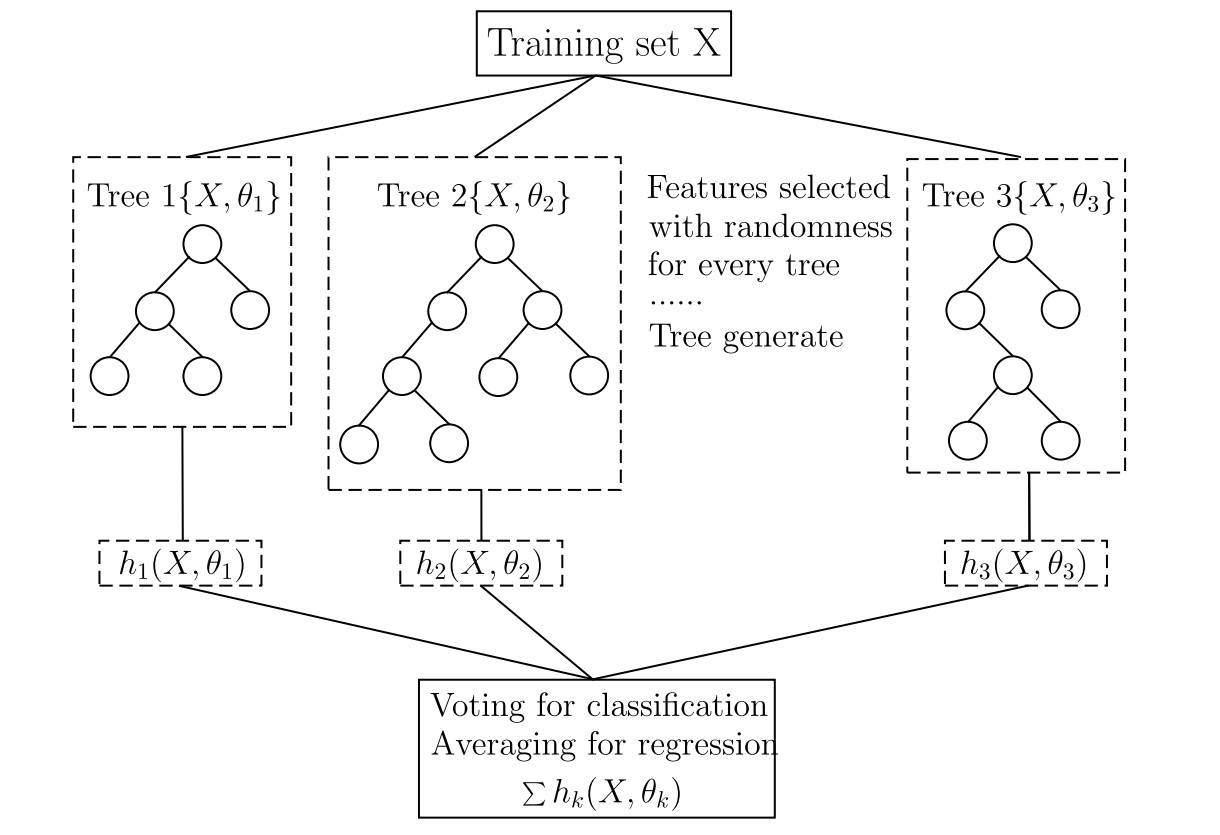
\includegraphics[width=\linewidth]{topics/chart.jpg}
	\caption{Fluxograma classificatório da florestas randômica, por \cite{Zhang2018}.}
	\label{fig:chartrandomforest}
\end{figure}



No caso do algoritmo, será feito uma análise dos dados, histórico para realização do treinamento do modelo, este modelo é composto de padrões matemáticos, ou seja, métricas gerais do comportamento histórico das informações. Com esses modelos gerados a partir de uma montanha de dados, será capaz o algoritmo realizar a predição de um novo dado, possibilitando a avaliação, por exemplo, de uma escolha boa ou ruim de determinado computador.
%\include{topics/problematica}
%\include{topics/classificador}
\chapter{\textbf{Conclusão}} % Este comando é utilizado para criar capítulos
A arquitetura de uma aplicação de IoT é composta por inúmeros desafios. Seu arranjo preserva os principais pilares dos sistemas distribuídos, como a disponibilidade, escalabilidade, confiabilidade e tolerância à falha, como descrito por \cite{vanSteen2016}\par
Existirá grandes desafios durante a elaboração desta arquitetura, para isso, será fundamental o estudo e pesquisa de novas tecnologias, a comparação entre os principais tipos de soluções  nas quais irá auxiliar para a execução desta arquitetura.\par
Ainda existem temas a serem abordados dentro do tema principal do trabalho, uma arquitetura publish/subscribe tornase essencial em uma arquitetura ideal em redes de dispositivos IoT.\par

%%% ====================================================================
%%% Início da parte pós-textual do documento.
\postextual


%%% Referências Bibliográfica

\bibliography{topics/bibliography}

%%%% Início dos apêndices ---------------------------------------------
\apendices


% --------------------------------------------------------------------
\chapter{Titulo}

\begin{enumerate}
    \item Item 1
    \item Item 2
\end{enumerate}

% --------------------------------------------------------------------



%%%% Início dos anexos ------------------------------------------------
\anexos

\partanexos*

\chapter{Exemplo de lombada}

\hspace*{0mm}\fbox{\includegraphics[scale=0.8]{pics/normas-ifes-apendice-d.png}}

\end{document}

